\chapter*{Introduction}
\addcontentsline{toc}{chapter}{Introduction}

\section*{What is \toolboxname?}
\addcontentsline{toc}{section}{What is \toolboxname?}

Lynx is a research-oriented MATLAB toolbox for supervised and semi-supervised learning. It is aimed at making the comparison of multiple learning algorithms \textit{fast} to implement, \textit{simple} to modify, and easily \textit{repeatable} by others.

Its main idea is summarized in Fig. \ref{fig:generalschema}. Instead of writing yourself the code to organize the comparison, you can specify its details in a human-understandable configuration file, which is loaded by Lynx. At this point, the toolbox takes charge of everything else: importing the requested datasets, partitioning them, running the algorithms, collecting the results and analyzing them. Moreover, it can distribute such simulations on multiple threads, and multiple computers, using the Parallel Computing Toolbox\footnote{\url{http://www.mathworks.it/products/parallel-computing/}} and the Distributed Computing Server\footnote{\url{http://www.mathworks.it/products/distriben/}} of MATLAB.

\begin{figure}[t]
\centering
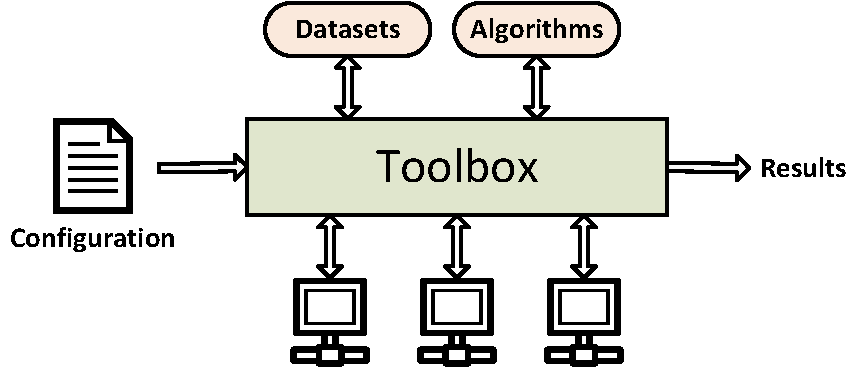
\includegraphics[scale=0.6]{./images/ToolboxSchema}
\caption{Schematic representation of the toolbox}
\label{fig:generalschema}
\end{figure}

In the configuration file, you can specify every detail of the simulation, including:

\begin{itemize}
\item the learning algorithms to use in the simulation,
\item which performance measures to compute (e.g. mean-squared error, ROC curves, etc.),
\item how to partition the data,
\item additional preprocessing steps for the datasets, or features for the algorithms (e.g. feature selection procedures),
\item enabling GPU support, saving the results, running a statistical test, and many other functionalities.
\end{itemize}

\section*{How do I read this manual?}

The strengths of Lynx, we hope, are more easily shown than said. Before starting, however, chapter \ref{chap:theoreticalbackground} summarizes briefly the essential concepts of supervised learning. Although most readers will be highly familiar with these, we use the chapter to introduce a small set of definitions around which the toolbox is organized, so we advise even the most experienced reader to a quick glimpse at the chapter.

Following this, chapter \ref{chap:install} details how to install the toolbox, and it contains a step-by-step guide to run two initial simulations. Then, chapter \ref{chap:writingconfig} and chapter \ref{chap:advancedfeatures} detail how to write your own configuration files, starting from the basic instructions (e.g. adding a dataset) up to the most advanced functionalities (e.g. parallelizing the experiments). Finally, it is time to develop your own classes: chapter \ref{chap:programminglynx} and chapter \ref{chap:advancedprogramming} present guided examples for implementing everything, including new learning algorithms, new performance measures, and even new learning tasks.

Additionally, we have included two appendices. Appendix \ref{chap:expfeatures} details experimental features we are working on, which have no support yet and that are expected to change rapidly over the course of the next months. Then, appendix \ref{chap:futuredevelopments} concludes by detailing some of other features we plan on implementing. We use this also to mention what we believe are the current ``weak'' points of the toolbox, that will require further development in the future.
